\chapter{Position Sizing}
\bichaptertitle{仓位规模设定}

LET'S COME BACK TO SERGEI'S THREE QUESTIONS FROM CHAPTER seven. First, how much do you like this trade? This is the forecast for each instrument. Secondly, how much can you afford to lose? You should know how many chips of trading capital you're willing to put down on the hypothetical casino baize depending on your desired target volatility. So far, so good. But how many shares, bonds, spread bet points or futures contracts should you actually buy or sell? What does a combined forecast of -6 and a £1,000,000 annualised cash target volatility mean in practice if you're trading crude oil futures in New York? To answer this we need to come back to Sergei's third question: how risky is your trade?

让我们回到第七章里 Sergei 提出的三个问题。第一，你有多看好这笔交易？这对应于每个品种的预测值。第二，你最多能承受多大亏损？
根据你想要达到的目标波动率，你应该知道自己愿意在那张假想赌场赌桌上押下多少筹码。到目前为止，一切都还说得通。
但实际操作中，你到底应该买入或卖出多少股票、债券、点差投注点数，或者多少期货合约？如果你在纽约交易原油期货，
那么一个合成预测值为 -6、年化现金目标波动率为 1,000,000 英镑，到底在实务上意味着什么？要回答这个问题，
我们就得回到 Sergei 的第三个问题：你的这笔交易到底有多大风险？

Once you know this you can move from the abstract world of forecasts and trading rules to deciding the size of actual positions in real financial instruments.

一旦弄清楚这一点，你就能够从预测值和交易规则的抽象世界，进入真实金融工具的实际仓位规模决策。

\section*{Chapter overview}
\phantomsection
\addcontentsline{toc}{section}{Chapter overview}
\bisectiontitle{本章概览}

\begin{tabularx}{\textwidth}{@{}p{0.30\textwidth}Y@{}}
\textbf{How risky is it?} & If you own one unit of an instrument how much risk does that expose you to? \\
\textbf{Volatility target and position risk} & What is the relationship between your cash volatility target and the risk of each instrument? \\
\textbf{From forecast to position} & Given how confident you are in your forecasts, the cash volatility target you have and the position risk, what size position should you be holding? \\
\end{tabularx}

\medskip

\begin{tabularx}{\textwidth}{@{}p{0.30\textwidth}Y@{}}
\textbf{风险有多大？} & 如果你持有一个单位的品种，这会让你暴露于多大风险之中？ \\
\textbf{波动率目标与} & 你的现金波动率目标，与每个品种本身的风险之间是什么关系？ 仓位风险 \\
\textbf{从预测到仓位} & 在你对预测的信心、你的现金波动率目标以及品种风险都已知的情况下， 你到底应该持有多大的仓位？ \\
\end{tabularx}

\section*{How risky is it?}
\phantomsection
\addcontentsline{toc}{section}{How risky is it?}
\bisectiontitle{风险有多大？}

What is the expected risk of holding an instrument?\footnote{Notice we're dealing here with expected, predictable risk, as discussed on page 39.\par 请注意，我们这里讨论的是预期的、可预测的风险，
正如第 39 页所讨论的那样。} If you own one Apple share or one crude oil futures contract, how much danger are you exposed to?

持有某个品种的预期风险是什么？如果你持有一股苹果股票，或者一份原油期货合约，那么你究竟暴露在多大风险之下？

\subsection*{Position block and block value}
\bisubsectiontitle{仓位单位与单位价值}

Let's start by asking a philosophical question. What exactly is ‘one' of an instrument? I define this as the instrument block. If ‘one' of an instrument goes up in price by 1\% how much do you gain or lose? This is the block value. These definitions will seem trivial to equity investors. ‘One' Apple share is exactly that -- one Apple share. If a share has a price of \$400 it will cost exactly \$400 to buy one block. If the price goes up by 1\% from \$400 to \$404 then you will gain \$4. Apple shares, and most other equities, have a natural instrument block of one share and a block value of 1\% of the price. Sometimes though to reduce costs you'll trade in larger blocks, usually of 100 shares. In this case the block value will be 100 × 1\% × share price, which is equal to the cost of one share. But life isn't always that simple. For example you can use a UK financial spread betting firm to bet on the FTSE falling at £10 a point. If the FTSE rises 1\% from 6500 to 6565 you would lose £650. Here the block value is ten times 1\% of the price. Futures contracts also have non-trivial block values. WTI crude oil futures on NYMEX are quoted in dollars per barrel. But each futures contract is for 1000 barrels. This means

我们先从一个哲学问题开始。某个品种的“一个单位”到底是什么意思？我把它定义为品种单位（instrument block）。
如果某个品种的“一个单位”价格上涨了 1\%，你会赚或亏多少钱？这就是单位价值（block value）。这些定义对股票投资者来说似乎不值一提。
苹果股票的“一个单位”，就是一股苹果股票。如果股价是 400 美元，那么买入一个单位的成本正好就是 400 美元。如果价格从 400 美元上涨 1\% 到 404 美元，
你就会赚 4 美元。苹果股票以及大多数其他股票，都天然地以一股作为品种单位，而它们的单位价值就是价格的 1\%。不过有时为了降低成本，
你会用更大的单位来交易，通常是 100 股。在这种情况下，单位价值就是 100 × 1\% × 股价，也就是一股价格对应的金额。但现实并不总是这么简单。
例如，你可以通过英国的金融点差投注公司，以每点 10 英镑的规模押注 FTSE 下跌。如果 FTSE 从 6500 上涨 1\% 到 6565，
你就会亏损 650 英镑。这里的单位价值就是价格 1\% 变动金额的 10 倍。期货合约也有并不那么直观的单位价值。
纽约商业交易所（NYMEX）的 WTI 原油期货报价单位是每桶多少美元，但每份期货合约对应的是 1000 桶原油。这意味着

a 1\% move up in price from \$75 to \$75.75 will net you \$750 on a long position of one contract, giving a block value of \$750. A Eurodollar future represents the cost of nominally borrowing \$1 million for three months and is priced at 100 minus the annual interest rate. If the price rises by 1\% from 98.00 to 98.98 then the rate of interest payable has fallen from 2\% to 1.02\%. Because three months is a quarter of a year you will have saved \$1 million × 0.98\% × 0.25 = \$2,450 in interest on your loan. The block value is \$2,450.110

如果价格从 75 美元上涨 1\% 到 75.75 美元，那么持有一份多头合约你就会赚到 750 美元，因此其单位价值就是 750 美元。
欧元美元期货（Eurodollar future）代表的是名义上借入 100 万美元、期限三个月的融资成本，其价格等于 100 减去年化利率。
如果价格从 98.00 上涨 1\% 到 98.98，那么应支付的利率就从 2\% 降到了 1.02\%。由于三个月是一年的四分之一，
你在这笔贷款上节省的利息就是 \$1 million × 0.98\% × 0.25 = \$2,450。它的单位价值就是 \$2,450。110

\subsection*{Price volatility}
\bisubsectiontitle{价格波动率}

We've established that a 1\% fall in quoted price will cause a certain degree of pain, equal to the block value, for each instrument block of an instrument that you're long. But how likely is a 1\% fall in price? Equity prices can easily change by 1\% or more in minutes, but a two-year bond might not see a 1\% move over several months. How should you take these different levels of risk into account? This is another job for volatility standardisation. You need to calculate an expected standard deviation of daily instrument percentage returns, which I'm going to define as the price volatility of an instrument. So for example the price volatility of an average equity is around 1\%, whereas as I write this the German two-year Schatz bond future has a daily standard deviation of just 0.02\%.

我们已经知道，对于你持有多头的每一个品种单位而言，报价下跌 1\% 会带来某种程度的痛苦，而这个痛苦的规模就等于单位价值。
但价格下跌 1\% 的概率有多大？股票价格在几分钟内就可能轻松波动 1\% 甚至更多，但一只两年期债券可能几个月都不会出现 1\% 的波动。
我们应该如何把这些不同层级的风险纳入考虑？这又是波动率标准化该出场的时候了。你需要计算品种日百分比收益的预期标准差，
我把它定义为该品种的价格波动率（price volatility）。例如，一只普通股票的价格波动率大约是 1\%，而在我写下这段话时，
德国两年期 Schatz 国债期货的日标准差仅仅只有 0.02\%。

CONCEPT: MEASURING RECENT STANDARD DEVIATION Remember that my standard definition of predictable risk (from page 39) is the expected daily standard deviation of prices. One of the simplest ways to estimate future volatility is to use a measure of recent standard deviation. This works surprisingly well because volatility tends to persist; if the market has been crazy over the last few weeks it will probably continue to be crazy for a few more weeks. I recommend using one of three methods to calculate recent standard deviation. The first method is to eyeball the chart. If you look at figure 22 you can see that the average daily change in crude oil futures over the last month of the chart is around \$1.0 a day, or 1.33\% of the final price of \$75. This method is fine for semi-automatic traders who will probably be staring at charts anyway, but I don't recommend it for others. The second method is to calculate the precise standard deviation of price changes over a moving window of time -- the volatility look-back period. You can use a

概念：衡量近期标准差 请记住，我对“可预测风险”的标准定义
（见第 39 页）是价格的预期日标准差。估计未来波动率最简单的方法之一，就是使用近期标准差的度量。之所以这种方法出奇地有效，
是因为波动率往往具有持续性；如果过去几周市场一直很疯狂，那么它在未来几周大概率仍然会很疯狂。我建议用三种方法之一来计算近期标准差。
第一种方法，是直接用眼睛看图。如果你看图 22，就会发现图表最后一个月里原油期货的平均日波动大约是每天 1.0 美元，也就是相对于最终价格 75 美元的 1.33\%。
这种方法对于半自动交易者来说没问题，因为他们本来就可能一直盯着图表看；但我并不推荐其他人这么做。第二种方法，
是用一个移动时间窗口
--- 也就是波动率回看期
--- 来精确计算价格变动的标准差。你可以使用一个

short window like ten business days (around two weeks), or a longer one such as 100 days. As the upper panel of figure 23 shows, shorter windows mean your volatility estimate is noisy, which as you'll see in chapter twelve will mean higher trading costs, but reacts very quickly to changes. The slower estimate is smoother, however it takes longer to adjust to new volatility environments. It's not obvious which look-back would be best. In my research I found almost no difference in performance before costs for lookback periods from a few days up to six months in length.111 Rather than risk overfitting I decided on a default look-back of 25 business days, or five weeks. This corresponds to the most popular value used across the industry, for example by the RiskMetrics (TM) system.112 I'll discuss in chapter twelve, ‘Speed and Size', when and why you'd use a longer look-back for instruments that are expensive to trade. The lower panel of figure 23 shows the volatility estimation using a 25 day lookback. It also shows the estimate coming from my third method, which is to use an exponential weighted moving average (EWMA) of standard deviation. This gives a smoother measure than a simple moving average that still reacts quickly to significant changes in the state of the market. I've chosen the default look-back for this as 36 days, which is equivalent to a 25 day window for a simple moving average.\footnote{The two measures have the same half-life when using a 25 day look-back for the simple moving average, and 36 days for exponentially weighted.\par 当简单移动平均使用 25 天回看期、
而指数加权使用 36 天回看期时，这两种度量具有相同的半衰期。} Details of how to calculate volatility with both kinds of moving average are shown in appendix D on page 298. Using recent price volatility is generally a good way to get the right risk adjusted position size. However it would be a disaster if you were using this method to trade Credit Default Swaps in early 2007, the front of the Eurodollar futures curve at any time in the US zero interest rate period, or for that matter Swiss franc FX in early January 2015. During all of these periods there was really low price volatility. If volatility is low then you would buy large numbers of instrument blocks, since each block has very little expected risk. But after periods of calm markets have a nasty habit of becoming crazy overnight, leaving you with dangerously large positions. As I've already mentioned in earlier chapters, holding very low volatility assets is generally a bad idea, and this is yet another reason to avoid them.

较短窗口，比如 10 个交易日
（约两周），也可以用较长窗口，比如 100 天。正如图 23 的上图所示，窗口越短，波动率估计就越噪声化，
而你会在第十二章看到，这意味着更高的交易成本，但它对变化的反应也会非常快。较慢的估计更平滑，不过适应新的波动环境也更慢。
到底哪种回看期最好，其实并不明显。我的研究发现，在扣除成本之前，从几天到六个月不等的回看期，在表现上几乎没有差别。111
为了避免过拟合风险，我把默认回看期设为 25 个交易日，也就是五周。这对应于业内最常见的取值，例如 RiskMetrics（TM）系统就采用这一思路。112
我会在第十二章“速度与规模”中讨论，对于交易成本高的品种，你为什么以及在什么情况下会使用更长的回看期。图 23 的下图展示了使用 25 天回看期的波动率估计。
它同时也展示了我第三种方法所得到的估计值，也就是使用标准差的指数加权移动平均（EWMA）。这种方法给出的估计比简单移动平均更平滑，
但仍能对市场状态的重大变化作出快速反应。我为这种方法选定的默认回看期是 36 天，这相当于简单移动平均的 25 天窗口。关于如何用这两种移动平均来计算波动率，
你可以在第 298 页的附录 D 中看到细节。使用近期价格波动率，通常是获得正确风险调整后仓位规模的好方法。然而，如果你在 2007 年初用这种方法去交易信用违约掉期，
或者在美国零利率时期的任何时间去交易欧元美元期货曲线前端，或者在 2015 年 1 月初去交易瑞郎外汇，那么结果就会是一场灾难。
因为在所有这些时期里，价格波动率都非常低。如果波动率很低，你就会买入大量品种单位，因为每个单位看起来都只有很小的预期风险。
但平静期过后，市场有个糟糕的习惯：它们会在一夜之间变得疯狂，而这会让你背上危险得多的超大仓位。正如我在前几章已经说过的那样，
持有超低波动资产通常是个坏主意，这里又提供了一个你应当避开它们的理由。

\begin{enumerate}
  \item Much slower than six months and performance gets steadily worse.
  \item As of 2015 RiskMetrics (TM) is owned by MSCI but it was originally developed by JP Morgan. It uses an exponentially weighted moving average whose half-life is equivalent to that of a 25 day simple moving average.
\end{enumerate}

\begin{enumerate}
  \item 如果比六个月更慢，表现就会持续变差。
  \item 截至 2015 年，RiskMetrics（TM）归 MSCI 所有，但它最初是由 JP Morgan 开发的。它采用的是指数加权移动平均，其半衰期等价于 25 天简单移动平均。
\end{enumerate}

\begin{figure}[htbp]
  \centering
  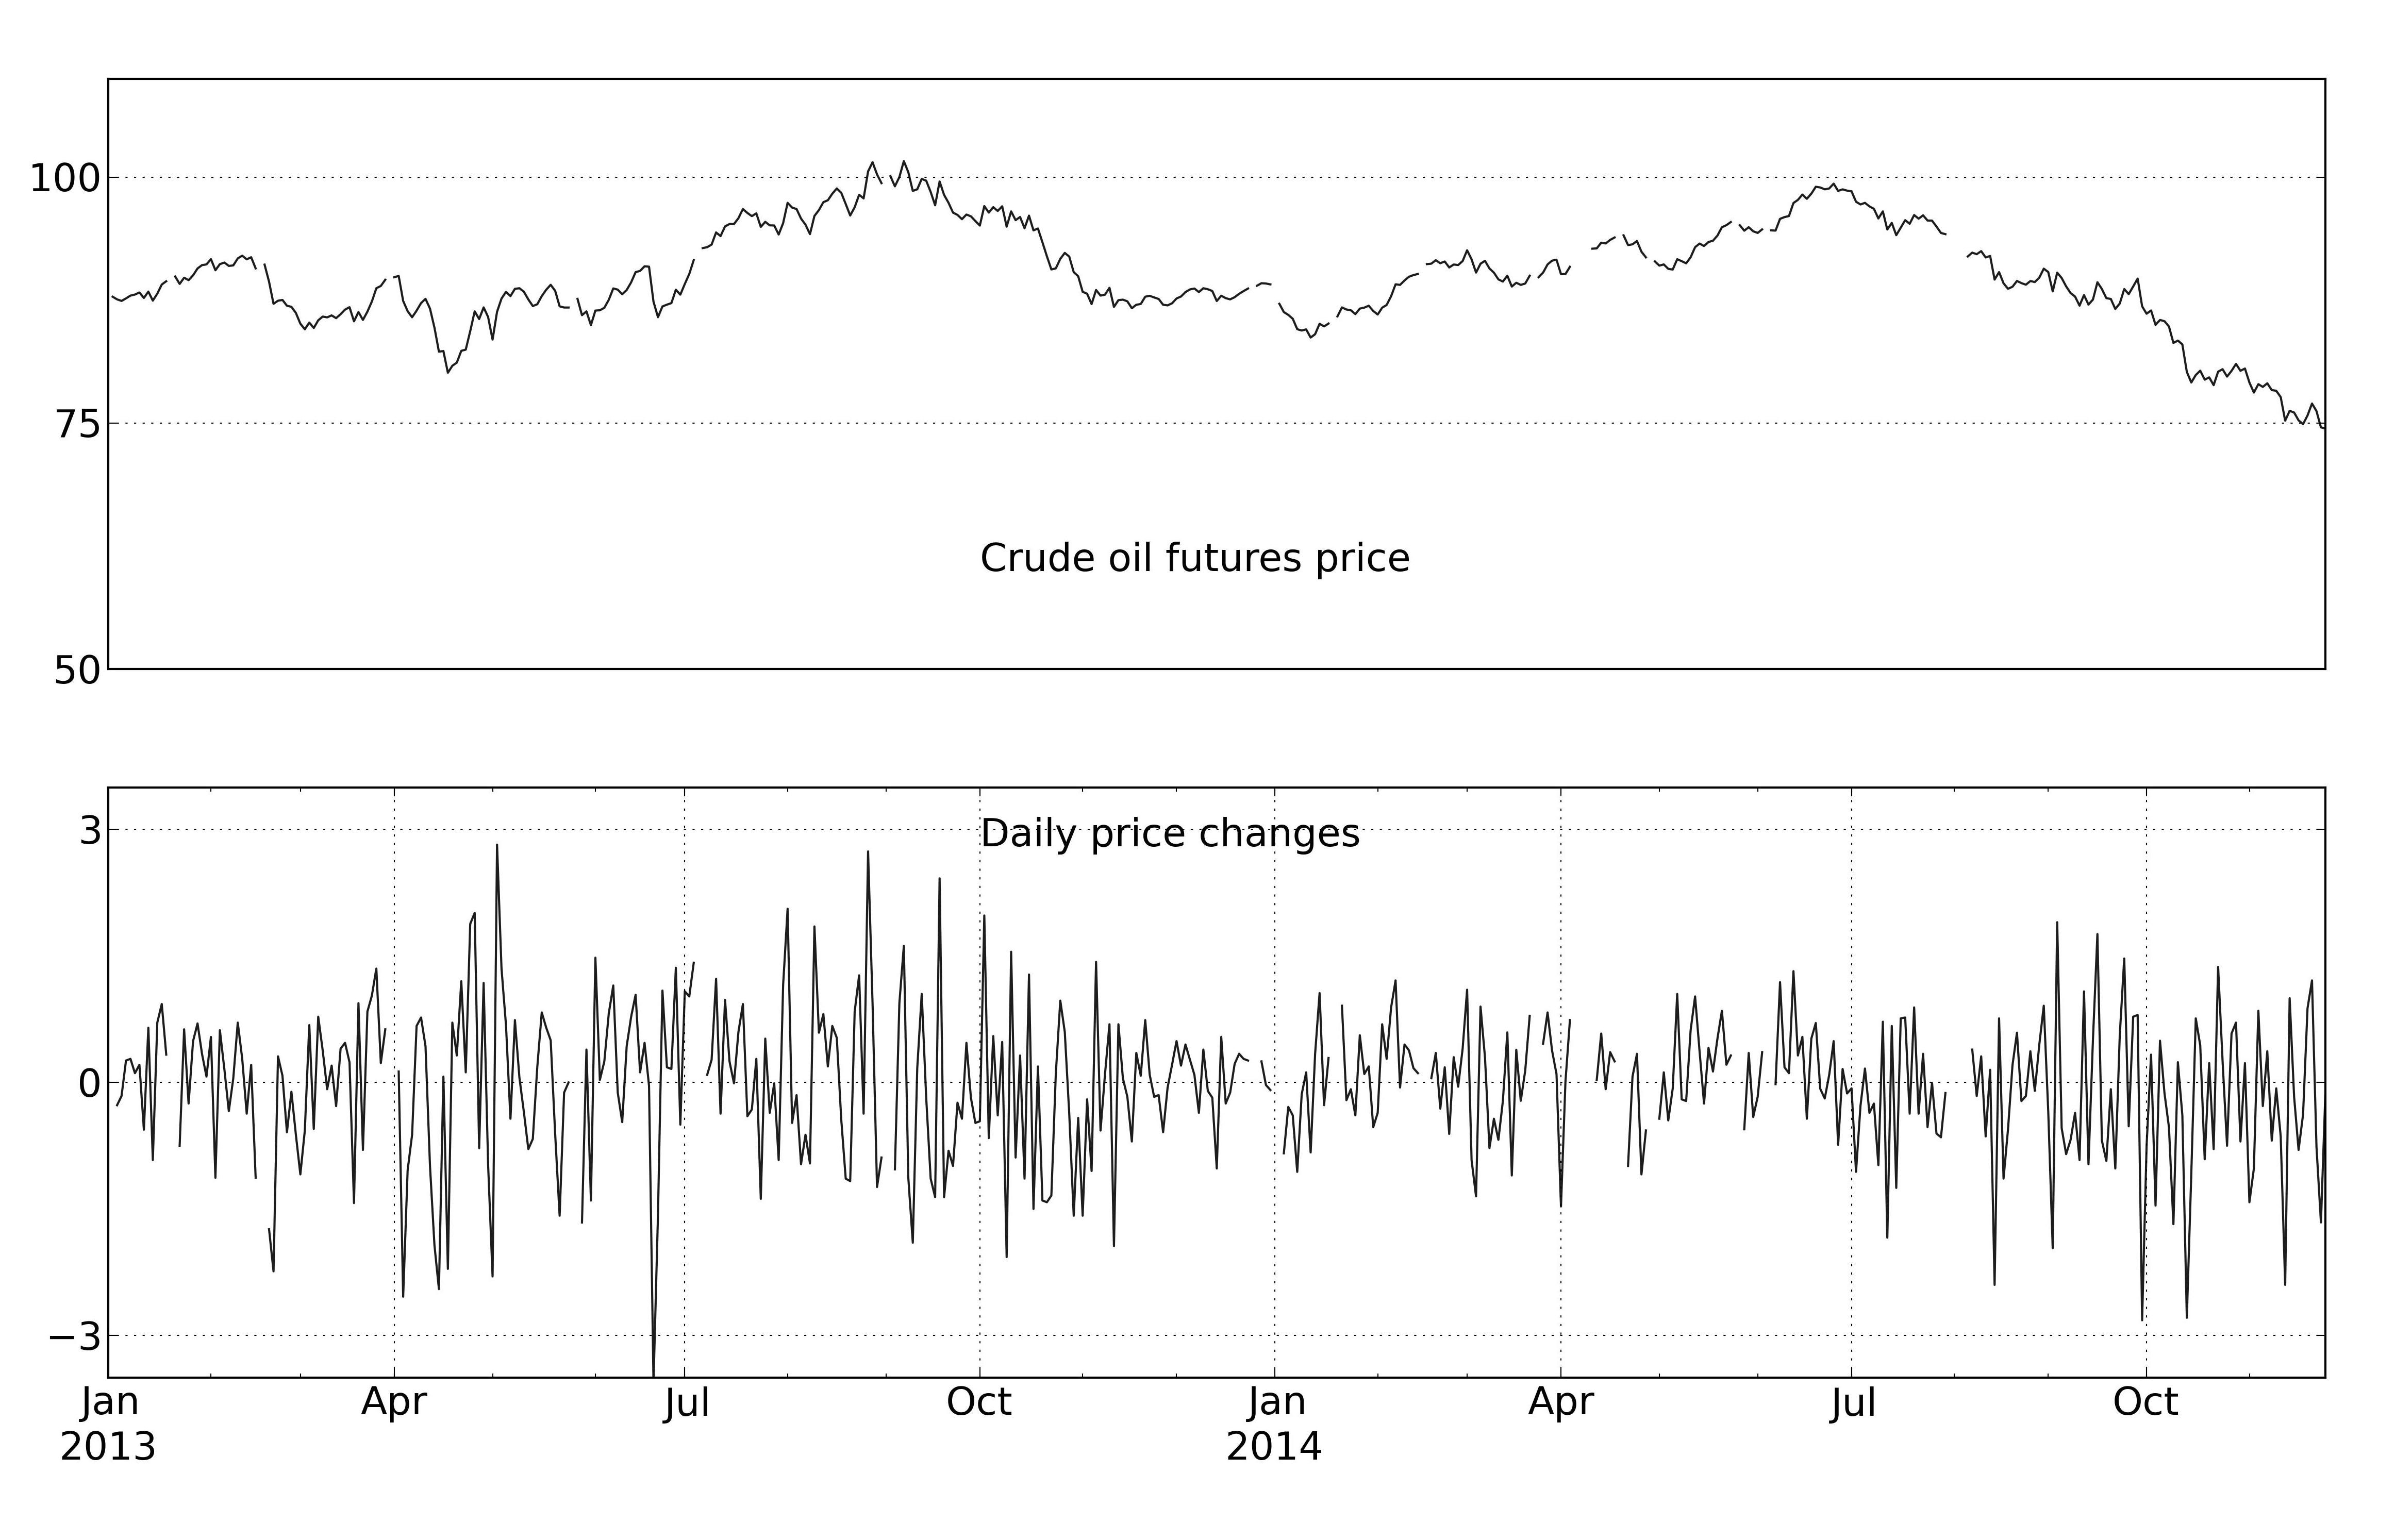
\includegraphics[width=\textwidth]{figures/raw/img-022.png}
  \caption{PRICE AND DAILY CHANGES IN CRUDE OIL FUTURES\\
  原油期货价格及其日度变化}
\end{figure}

\begin{figure}[htbp]
  \centering
  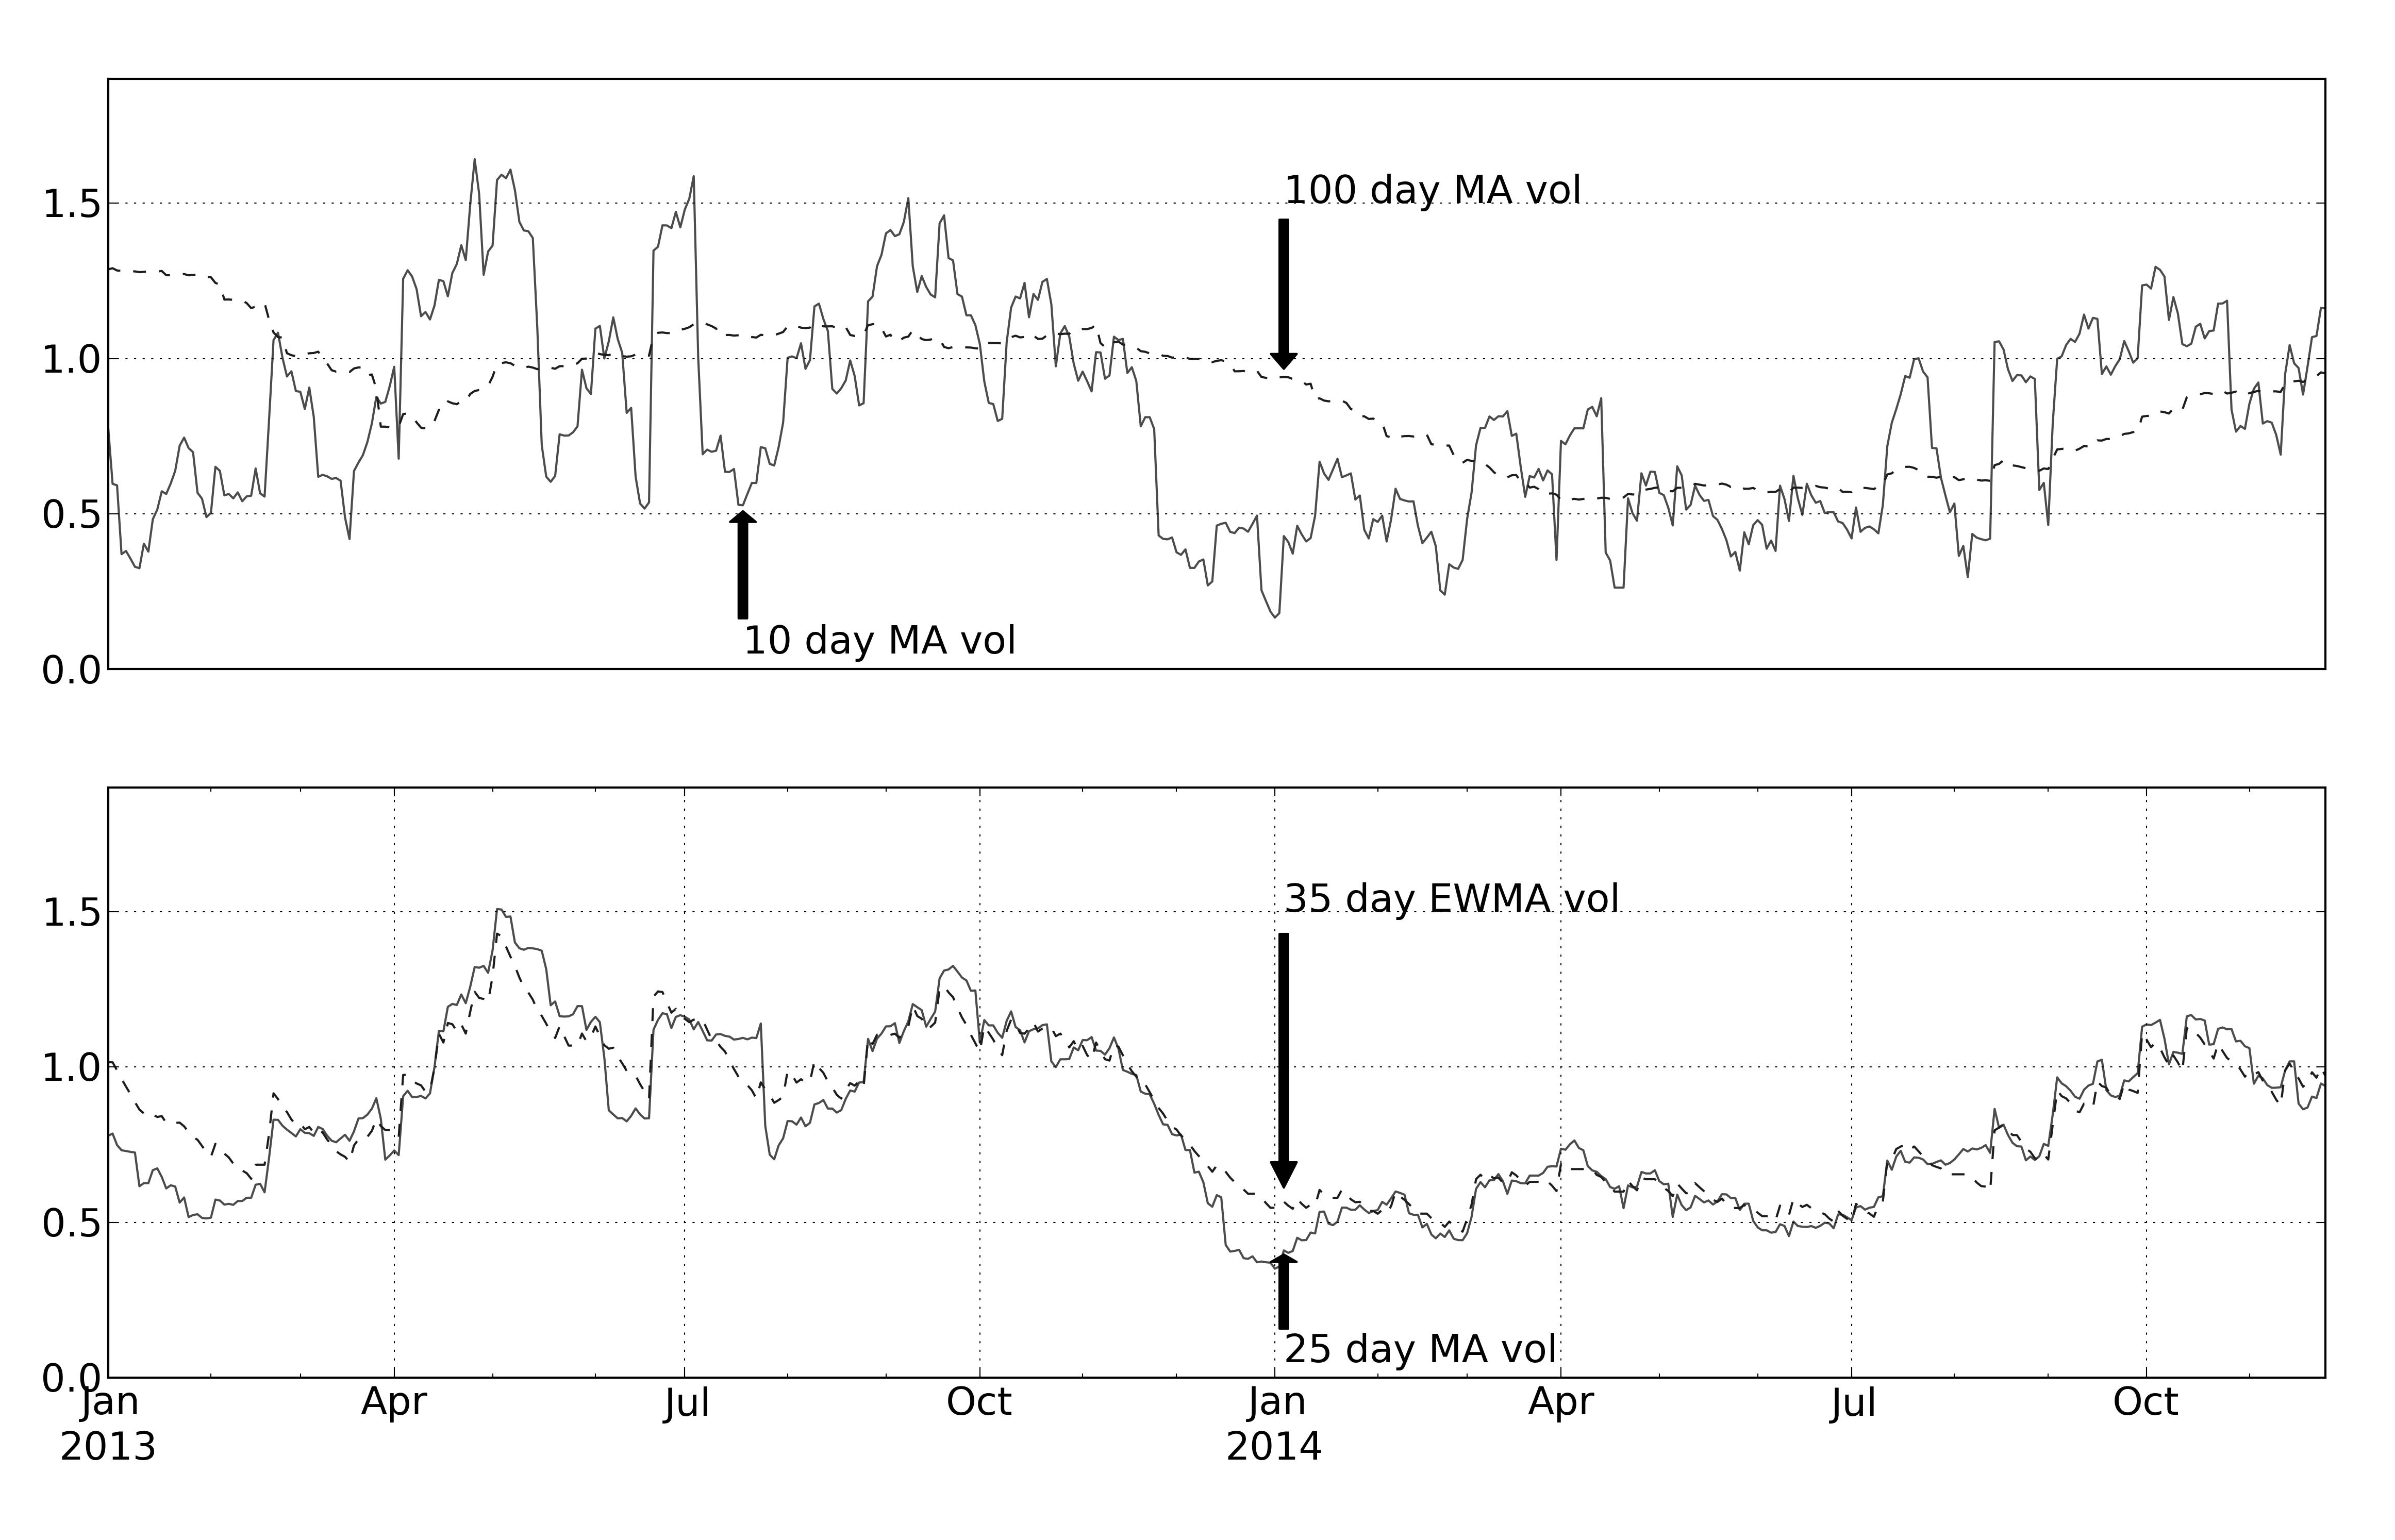
\includegraphics[width=\textwidth]{figures/raw/img-023.png}
  \caption{MEASURING CRUDE OIL PRICE VOLATILITY USING SIMPLE MOVING AVERAGE (MA) AND EXPONENTIALLY WEIGHTED (EWMA) STANDARD DEVIATIONS WITH VARIOUS LOOK- BACKS, IN DAYS\\
  使用不同天数回看期的简单移动平均（MA）与指数加权（EWMA）标准差来衡量原油价格波动率}
\end{figure}

Returning to the example I opened the chapter with, if you use the bottom panel of figure 23 the price volatility of crude oil futures here is around \$1 per day, which is 1.33\% of the final price shown (\$75).

回到本章开头的例子。如果你使用图 23 的下图，那么这里原油期货的价格波动率大约是每天 1 美元，也就是相对于最终显示价格 75 美元的 1.33\%。

\subsection*{Instrument currency volatility}
\bisubsectiontitle{品种货币波动率}

If one oil futures contract has a block value of \$750, and a price volatility of 1.333\%, then what is the risk of owning one contract? This is the instrument currency volatility; it's the expected standard deviation of daily returns from owning one instrument block in the currency of the instrument. For oil futures you'd expect on any given day to see a price move of around 1.33\% and since each 1\% price move will cost you \$750, your daily profit or loss will average around 1.33 × \$750 = \$997.50. So the instrument currency volatility for WTI crude oil futures is \$997.50. This value shouldn't be rounded. In general instrument currency volatility is equal to the block value multiplied by the price volatility. It will be in the same currency in which the block value is measured.

如果一份原油期货合约的单位价值是 750 美元，而价格波动率是 1.333\%，那么持有一份合约的风险是多少？
这就是品种货币波动率（instrument currency volatility）；它表示以该品种计价货币衡量时，持有一个品种单位所带来的日收益预期标准差。
对于原油期货而言，你预期任意一天价格会波动大约 1.33\%，而每 1\% 的价格波动会让你盈亏 750 美元，因此你的日利润或亏损平均大约会是
1.33 × 750 美元 = 997.50 美元。所以，WTI 原油期货的品种货币波动率就是 997.50 美元。这个值不应当被四舍五入。
一般来说，品种货币波动率等于单位价值乘以价格波动率。它的货币单位与单位价值所采用的计价货币相同。

\subsection*{What's that in real money?}
\bisubsectiontitle{折算成你真正账户里的钱是多少？}

This is all fine if you are a US investor trading crude oil futures, a Brit trading UK equities, or a Euro area investor buying German bonds. However many investors and traders will want to buy and sell in currencies that are different from their trading capital. The instrument currency volatility isn't good enough. Instead you need to know the volatility of the instrument value in the currency of your account, which will be the same currency as your cash volatility target. I call this the instrument value volatility. The instrument currency volatility needs to be converted to an instrument value volatility using an appropriate exchange rate. The exchange rate will have the currency of the instrument as the numerator, and the account value currency as the denominator. As an example for a UK investor with a GBP account, the instrument currency volatility of a crude oil future (\$997.50) will need to be multiplied by the current USD/GBP exchange rate, to work out what those dollars are worth in British pounds. As I write this paragraph the USD/GBP rate is 0.67, giving an instrument value volatility of \$997.50 × 0.67 = £668.325. Again you shouldn't round any numbers yet. Note I'm using USD/GBP, rather than GBP/USD which is normally quoted. Be sure you are using the correct rate.

如果你是美国投资者交易原油期货、英国人交易英国股票，或者欧元区投资者买入德国债券，那么上面的计算就够用了。
但很多投资者和交易者会用与自身交易资本不同的货币去买卖资产。在这种情况下，品种货币波动率就不够用了。你真正需要知道的，
是这个品种在你账户计价货币中的价值波动率，而这也将与你的现金波动率目标使用同一种货币。我把它称为品种价值波动率
（instrument value volatility）。要得到它，就需要用合适的汇率把品种货币波动率换算过来。这个汇率的分子应是品种的计价货币，
分母则是账户价值的计价货币。举个例子，对于一个以英镑为账户货币的英国投资者来说，原油期货的品种货币波动率为 997.50 美元，
那就需要乘以当前的 USD/GBP 汇率，才能算出这些美元折合成多少英镑。在我写下这一段时，USD/GBP 汇率大约是 0.67，
于是品种价值波动率就是 997.50 美元 × 0.67 = 668.325 英镑。同样地，在这一步你也不应当先行四舍五入。请注意，
我使用的是 USD/GBP，而不是平常更常见的 GBP/USD 报价。务必确认你使用的是正确方向的汇率。

\section*{Volatility target and position risk}
\phantomsection
\addcontentsline{toc}{section}{Volatility target and position risk}
\bisectiontitle{波动率目标与仓位风险}

Now let's relate this back to your cash volatility target -- the risk you require and are comfortable with from your trading account. From the previous chapter on volatility targeting (page 137) your daily cash volatility target is your long-term expected daily standard deviation of returns, measured in the currency of your trading capital.

现在，让我们把这一切重新和你的现金波动率目标联系起来
--- 也就是你希望自己的交易账户承担、且自己也能承受的风险水平。根据上一章关于波动率目标
（第 137 页）的定义，你的日现金波动率目标，就是以你的交易资本货币计量的、长期预期日收益标准差。

Let's refer back to the example I opened the chapter with. We had an investor with a £1,000,000 annualised cash target volatility, implying a daily target of one-sixteenth of that, £62,500.\footnote{Remember to go from annual to daily volatility you divide by the ‘square root of time'. As there are roughly 256 business days in a year, the appropriate divisor is 16.\par 记住，从年化波动率换算到日波动率时，
你需要除以“时间平方根”。由于一年大约有 256 个交易日，因此合适的除数是 16。} I worked out above that the crude oil future had an instrument value volatility of £668.325 for a UK investor. This is the daily risk of owning one instrument block -- a single futures contract. How many of these blocks of crude oil should this investor hold? For now let's assume we are putting together a trading subsystem for the investor; a trading system which only has a single instrument. We'll be achieving the entire cash volatility target by having positions in just one instrument; in this case crude oil. This assumption will be relaxed in the next chapter, when we look at creating a portfolio of subsystems. We also assume that we get the required target risk by having a constant amount of expected volatility from owning a fixed long position in the asset. So we won't worry yet about the value of any forecast for the instrument. I'll consider forecasts in the next section of this chapter. For the investor in the example to get the entire required daily standard deviation of £62,500 from being long crude oil futures they need to buy £62,500, divided by the risk of one contract, £668.325, or 93.52 contracts. The value of 93.52 is a scaling factor which accounts for the difference between an instrument's natural volatility and the required volatility of the portfolio. I call it the volatility scalar. In general the volatility scalar is equal to your daily cash volatility target, divided by the instrument value volatility. You'll notice that both of these variables are in the same currency as your trading capital. Also please note that you should not round the volatility scalar to a whole number.

让我们回到本章开头的那个例子。我们当时面对的是一位年化现金目标波动率为 1,000,000 英镑的投资者，这意味着其日目标波动率是其十六分之一，
也就是 62,500 英镑。上面我已经算出，对于一位英国投资者来说，原油期货的品种价值波动率是 668.325 英镑。这个值就是持有一个品种单位
--- 一份期货合约
--- 所带来的日风险。那么，这位投资者应当持有多少份这样的原油期货单位呢？现在我们先假设，我们正在为这位投资者构建一个交易子系统；
也就是说，这是一套只包含单一品种的交易系统。我们将通过只持有一个品种
--- 这里就是原油
--- 的仓位，来实现全部现金波动率目标。这个假设会在下一章被放松；届时我们将讨论如何构建由多个子系统组成的投资组合。
我们还假设，我们是通过持有某个资产的固定多头仓位，让预期波动率保持恒定，从而达到所要求的目标风险。因此，我们暂时先不考虑该品种预测值的影响。
本章下一节才会讨论预测值。在这个例子里，要让这位投资者仅靠持有原油期货多头，就达到所需的 62,500 英镑日标准差，
他需要买入 62,500 英镑 ÷ 668.325 英镑 = 93.52 份合约。93.52 这个数字，就是一个缩放因子，它反映了品种天然波动率与投资组合所需波动率之间的差异。
我把它称为波动率缩放因子（volatility scalar）。一般来说，波动率缩放因子等于你的日现金波动率目标除以品种价值波动率。
你会注意到，这两个变量都使用和你的交易资本相同的货币计量。同时也请注意，你不应当把波动率缩放因子先四舍五入为整数。

\section*{From forecast to position}
\phantomsection
\addcontentsline{toc}{section}{From forecast to position}
\bisectiontitle{从预测到仓位}

I've shown that the investor in the simple example for this chapter would need to own a long position in 93.52 crude oil futures (the volatility scalar) to realise their desired volatility target. This however ignores any forecast that the investor has made; either a combined forecast from multiple trading rules, or the single forecasts made by asset allocating investors and semi-automatic traders. At the start of the chapter I'd assumed that the forecast is -6 in the example. Clearly the investor is going to want to be short, rather than long, but by how much? To work this out you need to think about average forecasts. Over a long period of time you'll still want to be hitting your volatility target for returns, no matter what your daily forecasts are. In chapter seven (page 112) I recommended that forecasts should have a

我已经展示过：在本章的简单例子里，这位投资者如果想达到自己的目标波动率，就需要持有 93.52 份原油期货的多头仓位
（也就是波动率缩放因子）。不过，这一计算忽略了投资者自己的预测值，无论这个预测值是由多条交易规则合成得出的，还是资产配置型投资者、
半自动交易者所给出的单一预测值。本章开头我假设，这个例子的预测值是 -6。显然，这位投资者会想做空，而不是做多，但到底该空多少？
要算出这一点，你需要思考“平均预测值”这个概念。从长期来看，无论你的日常预测值如何变化，你都仍然希望自己的收益能够达到既定波动率目标。
在第七章
（第 112 页）中，我建议预测值应当具有

long run average absolute value of 10. This implies that to hit your target over the long run you'd want your positions to have the same average expected variation as if you had a constant forecast of +10. Effectively then the volatility scalar gives you a position which is consistent with having a constant forecast of +10. If you're currently more optimistic with a larger positive forecast you should buy more blocks; and if you're pessimistic you should have fewer blocks, or go short if the forecast is negative. In the example above I calculated a volatility scalar of 93.52 crude oil futures contracts. This will be consistent with the long run forecast, so a forecast of +10 equates to buying 93.52 contracts (ignoring for the moment that you can't hold fractional contracts). If the forecast falls to +5 you'd only be half as confident, and want half the original position, 46.76 contracts. A forecast of -20 would mean you'd want to go short twice the original position, a sell of 187.04 blocks. The resulting quantity of blocks is the subsystem position. It's a subsystem position because, as I said earlier, we're assuming in this chapter your entire capital is invested in a subsystem trading one instrument, rather than in a complete trading system running across a number of instruments. A subsystem position is equal to the volatility scalar multiplied by the forecast, then divided by the long average of 10. So for the crude oil example with a forecast of -6, and where I've worked out the volatility scalar to be 93.52, the subsystem position will be (93.52 × -6) ÷ 10 = -56.11, implying a short of 56.11 contracts. Again you shouldn't do any rounding of non integer positions for now. If you're an asset allocating investor you've probably spotted that with a constant forecast which is always equal to +10 (from the single ‘no-rule' rule), your position will always be equal to the volatility scalar. For other traders and investors your position will depend on your forecast and on the components of the volatility scalar (your cash volatility target for your portfolio and the account value volatility of the instrument). Higher absolute forecasts, bigger account sizes, a greater appetite for risk and lower instrument price volatility will mean larger positions; and vice versa.

长期平均绝对值为 10。这意味着，如果你想在长期内达到目标，那么你的仓位平均预期波动幅度应当与“预测值恒定为 +10”时相同。
从这个角度来看，波动率缩放因子给出的，其实就是一个与恒定预测值 +10 相一致的仓位。如果你当前更乐观、正向预测更大，
那你就应该买入更多单位；如果你更悲观，那你就应该持有更少单位，或者在预测为负时转为做空。在上面的例子中，
我算出的原油期货波动率缩放因子是 93.52 份合约。这个值与长期平均预测相一致，因此预测值为 +10 就对应买入 93.52 份合约
（暂且忽略你实际上无法持有小数份合约这一点）。如果预测值降到 +5，那就表示你的信心只有原来的一半，因此你想持有原始仓位的一半，
也就是 46.76 份合约。如果预测值是 -20，那就意味着你想做空原始仓位的两倍，也就是卖出 187.04 个单位。由此得到的品种单位数量，
就是子系统仓位（subsystem position）。之所以称为子系统仓位，是因为正如前面所说，在本章中我们假设你的全部资本都投入在一个只交易单一品种的子系统中，
而不是分散到一个跨多个品种运行的完整交易系统里。子系统仓位等于波动率缩放因子乘以预测值，再除以长期平均值 10。
因此，在原油这个例子里，预测值是 -6，而波动率缩放因子是 93.52，那么子系统仓位就是
(93.52 × -6) ÷ 10 = -56.11，也就是做空 56.11 份合约。同样地，在这一步你也不应对非整数仓位进行四舍五入。
如果你是一名资产配置型投资者，你大概已经发现：由于你的预测值恒定地等于 +10
（来自那条单一的“无规则”规则），那么你的仓位永远都会等于波动率缩放因子。对于其他交易者和投资者而言，
你的仓位则取决于预测值，以及波动率缩放因子的各个组成部分
（也就是投资组合的现金波动率目标与品种账户价值波动率）。预测值绝对值越大、账户规模越大、风险偏好越强，且品种价格波动率越低，
仓位就会越大；反之亦然。

\section*{Summary for position sizing}
\phantomsection
\addcontentsline{toc}{section}{Summary for position sizing}
\bisectiontitle{仓位规模设定总结}

Instrument Staunch systems traders: This is the combined forecast calculated in forecast chapter eight by weighting your trading rule forecasts for an instrument and accounting for the forecast diversification multiplier. Asset allocating investors: Equal to a constant value of +10. Semi-automatic traders: Single discretionary forecast. All groups will end up with one forecast per instrument. It will have an expected average absolute value of 10 and it is limited to a range of -20 to +20.

品种预测 坚定的系统化交易者：这是在第八章中通过对某个品种的各交易规则预测值加权、并考虑预测分散化乘数后得到的合成预测。
资产配置型投资者：恒定等于 +10。半自动交易者：单一主观预测。所有群体最终都会为每个品种得到一个预测值。
它的预期平均绝对值为 10，范围被限制在 -20 到 +20 之间。

Annualised This is the percentage volatility target multiplied by the trading capital, cash volatility from chapter nine. It's an annualised measure of expected risk from your target portfolio. It will be in units of the currency your trading capital is in.

年化现金波动率目标 这是第九章中的百分比波动率目标乘以交易资本得到的结果。它是目标投资组合预期风险的年化度量，
使用的是你的交易资本所对应的货币单位。

Daily cash Annualised cash volatility target divided by ‘the square root of time'; with volatility approximately 256 business days in a year you should divide by 16. target

日现金波动率目标 年化现金波动率目标除以“时间平方根”；由于一年大约有 256 个交易日，因此你应当除以 16。

Price Expected daily standard deviation of instrument price changes. Watch out volatility for very low standard deviations. It will be in units of percentage of price.

价格波动率 这是品种价格变动的预期日标准差。要特别小心那些标准差极低的品种。它以价格百分比为单位。

Instrument This is the size you trade instruments in. For equities this would usually block be one share, though 100 shares might make sense if trading fewer is uneconomic. For futures this will be a single contract and for spread bets it is the minimum bet per point.

品种单位 这是你实际进行交易时所使用的单位规模。对股票来说，通常是一股；不过如果交易少于 100 股不划算，那么 100 股也可能更合理。
对于期货来说，它就是一份合约；对于点差投注来说，则是每一点的最小下注额。

Block value This is how much each 1\% change in the price of a block translates into monetary value. It will be in units of instrument currency, i.e. \$ for US equities.

单位价值 这是指品种单位价格每变动 1\% 时，会转化成多少货币盈亏。它使用品种本身的计价货币，例如美国股票就是美元。

Instrument This is the daily standard deviation of instrument value. Equal to block value currency multiplied by the price volatility. It will be in units of instrument currency. volatility

品种货币波动率 这是品种价值的日标准差。它等于单位价值乘以价格波动率，使用品种货币单位计量。

Exchange This is the exchange rate between instrument currency (numerator) and the rate currency your trading capital is in (denominator).

汇率 这是品种货币
（分子）与交易资本货币
（分母）之间的汇率。

Instrument Daily standard deviation of instrument value, measured in your trading value capital currency. Equal to instrument currency volatility multiplied by the volatility exchange rate. It will be in units of your account currency.

品种价值波动率 这是以你的交易资本货币计量的品种价值日标准差。它等于品种货币波动率乘以汇率，结果使用你的账户货币单位。

Volatility Number of position units to hold if you are investing your entire trading scalar capital in one instrument, ignoring forecasts. Equal to daily cash volatility target divided by the instrument value volatility, both in your currency. It's in units of position blocks.

波动率缩放因子 如果你把全部交易资本都投入到单一品种中、并忽略预测值，那么你应持有多少个仓位单位。它等于日现金波动率目标除以品种价值波动率，
两者都使用你的账户货币计量。它的单位是品种单位数。

Subsystem How many blocks do you need to hold given your forecast? Equal to the position instrument forecast, multiplied by volatility scalar, divided by 10. This is in units of position blocks.

子系统仓位 在给定预测值的情况下，你应当持有多少个品种单位？它等于品种预测值乘以波动率缩放因子，再除以 10。单位是品种单位数。

\subsection*{Worked example for position sizing}
\bisubsectiontitle{仓位规模设定的完整示例}

From the start of the chapter the investor in this example has an annualised £1,000,000 volatility target and is investing in WTI Crude oil futures contracts, with a forecast of -6.

在本章开头的示例中，这位投资者的年化波动率目标是 1,000,000 英镑，投资对象是 WTI 原油期货合约，预测值为 -6。

Instrument -6 forecast

品种预测 -6

Annualised £1,000,000 cash volatility target

年化现金波动率目标 1,000,000 英镑

Daily cash Annualised cash volatility target divided by 16: £62,500 volatility target

日现金波动率目标 年化现金波动率目标除以 16：62,500 英镑

Price For crude oil the bottom panel of figure 23 shows average returns of \$1 a volatility day, which with a price of \$75 equates to 1.33\%.

价格波动率 对原油而言，图 23 的下图显示平均日波动约为 1 美元，而在价格为 75 美元时，这相当于 1.33\%。

Instrument One futures contract block

品种单位 一份期货合约

Block value For a WTI Crude contract of 1000 barrels with price \$75 a 1\% price move will equate to \$0.75 × 1000 = \$750.

单位价值 对于一份 1000 桶、价格为 75 美元的 WTI 原油合约，1\% 的价格变动等于 \$0.75 × 1000 = \$750。

Instrument This is the block value multiplied by the price volatility. currency For crude this is \$750 × 1.33 = \$997.50 volatility

品种货币波动率 这等于单位价值乘以价格波动率。对于原油而言，就是 \$750 × 1.33 = \$997.50。

Exchange Numerator is instrument currency, USD. Denominator is account value rate currency, GBP. The USD/GBP exchange rate is currently around 0.67.

汇率 分子是品种货币 USD，分母是账户价值货币 GBP。当前 USD/GBP 汇率大约是 0.67。

Instrument This is the instrument currency volatility multiplied by the exchange rate. value \$997.50 × 0.67 = £668.325 volatility

品种价值波动率 这等于品种货币波动率乘以汇率。\$997.50 × 0.67 = £668.325。

Volatility Daily cash volatility target divided by the instrument value volatility, both in scalar the investor's currency. £62,500 divided by £668.325 equals 93.52 contracts.

波动率缩放因子 以投资者账户货币计量的日现金波动率目标除以品种价值波动率。£62,500 ÷ £668.325 = 93.52 份合约。

Subsystem Final combined instrument forecast, multiplied by volatility scalar, then position divided by 10. (-6 × 93.52) ÷ 10 = short 56.11 contracts (no rounding).

子系统仓位 最终合成品种预测值乘以波动率缩放因子，再除以 10。(-6 × 93.52) ÷ 10 = 做空 56.11 份合约
（不做四舍五入）。

You can now answer all of Sergei's questions and you've finally got positions for a trading system that has a single instrument, the subsystem position. But any good trading system will have multiple assets and even semi-automatic traders normally have more than one bet on the table at a time. The next chapter examines how you can put several subsystems together into a portfolio.

现在你已经能够回答 Sergei 的全部问题，并且终于得到了一个只包含单一品种的交易系统所应持有的仓位，也就是子系统仓位。
但任何优秀的交易系统都会包含多个资产，而即便是半自动交易者，通常也会同时摆出不止一笔赌注。下一章将讨论，如何把多个子系统组合成一个投资组合。
